\documentclass{article}
\usepackage[utf8]{inputenc}
\usepackage[a4paper, total={6.5in, 9.5in}]{geometry}
\usepackage[bookmarks,hidelinks]{hyperref}
\usepackage{amsmath, amssymb}
\usepackage{float}
\usepackage{cancel}
\usepackage{multirow}
\usepackage{tikz}
\usepackage{caption}
\usepackage{calc}  
\usepackage{enumitem}  
\usepackage{graphicx}
\usepackage{scalerel,stackengine}
\stackMath
\newcommand\reallywidehat[1]{%
\savestack{\tmpbox}{\stretchto{%
  \scaleto{%
    \scalerel*[\widthof{\ensuremath{#1}}]{\kern-.6pt\bigwedge\kern-.6pt}%
    {\rule[-\textheight/2]{1ex}{\textheight}}%WIDTH-LIMITED BIG WEDGE
  }{\textheight}% 
}{0.5ex}}%
\stackon[1pt]{#1}{\tmpbox}%
}
\parskip 1ex
\graphicspath{ {./} }
\usetikzlibrary{shapes.arrows}
\let\ce\ch
\newcommand{\im}{\text{Im}\,}
\newcommand{\re}{\text{Re}\,}
\newcommand{\img}{\text{Img}\,}
\newcommand{\R}{\mathds{R}}
\newcommand{\C}{\mathds{C}}
\newcommand{\N}{\mathds{N}}
\newcommand{\Z}{\mathds{Z}}
\newcommand{\conj}[1]{\overline{#1}}
\newcommand{\Aff}{\text{Aff}}
\newcommand{\oo}{\infty}
\newcommand{\twoRows}[1]{\multirow{2}{*}{#1}}
\newcommand{\threeRows}[1]{\multirow{3}{*}{#1}}
\newcommand{\twoCols}[1]{\multicolumn{2}{c|}{#1}}
\newcommand{\threeCols}[1]{\multicolumn{3}{|c|}{#1}}
\newcommand{\twoColsNB}[1]{\multicolumn{2}{c}{#1}}
\newcommand{\goesto}[2]{\xrightarrow[#1\:\to\:#2]{}}
\newcommand{\liminfty}{\lim_{x\to+\oo}}
\newcommand{\limminfty}{\lim_{x\to-\oo}}
\newcommand{\limzero}{\lim_{x\to0}}
\newcommand{ \const}{\text{cste}}
\newcommand{\et}{\:\text{et}\:}
\newcommand{\ou}{\:\text{ou}\:}
\newcommand{\placeholder}{\diamond}
\newcommand{\mediateur}{\:\text{med}\:}
\newcommand{\milieu}{\:\text{mil}\:}
\newcommand{\vect}[1]{\overrightarrow{#1}}
\newenvironment{descriptiona}{\begin{description}[leftmargin=!,labelwidth=\widthof{\bfseries The longest label}]}{\end{description}}
\renewcommand{\arraystretch}{1.4}
\newcommand{\point}[2]{(#1;\;#2)}
\newcommand{\spacepoint}[3]{\begin{pmatrix}#1\\#2\\#3\end{pmatrix}}
\newcommand{\bijections}{%
	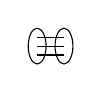
\begin{tikzpicture}[scale=1.5, baseline=-0.5ex]%
		\draw (-0.75ex,0) ellipse (0.5ex and 1ex);
		\draw (0.75ex,0) ellipse (0.5ex and 1ex);
		\draw (-0.75ex,0.5ex) -- (0.75ex,0.5ex);
		\draw (-0.75ex,0) -- (0.75ex,0);
		\draw (-0.75ex,-0.5ex) -- (0.75ex,-0.5ex);
	\end{tikzpicture}\,%
}

\newcommand{\injections}{%
	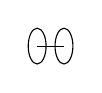
\begin{tikzpicture}[scale=1.5, baseline=-0.5ex]%
		\draw (-0.75ex,0) ellipse (0.5ex and 1ex);
		\draw (0.75ex,0) ellipse (0.5ex and 1ex);
		\draw (-0.75ex,0) -- (0.75ex,0);
	\end{tikzpicture}\,%
}

\newcommand{\surjections}{%
	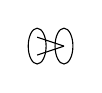
\begin{tikzpicture}[scale=1.5, baseline=-0.5ex]%
		\draw (-0.75ex,0) ellipse (0.5ex and 1ex);
		\draw (0.75ex,0) ellipse (0.5ex and 1ex);
		\draw (-0.75ex,0.5ex) -- (0.75ex,0);
		\draw (-0.75ex,-0.5ex) -- (0.75ex,0);
	\end{tikzpicture}\,%
}
\newcommand{\cP}{\mathcal{P}}
\newcommand{\fimd}{f^{\to}}
\newcommand{\fimr}{f^{\from}}
\newcommand{\compl}{\:^c\,\!\!}
\newcommand{\explain}[1]{\qquad\qquad\text{#1}}
\title{Exercices: Ordre supérieur}
\author{Ewen Le Bihan}
\date{2020-01-20}

\begin{document}
\maketitle

\abstract{}
\emph{Sujet disponible à \url{http://mpsi.daudet.free.fr/maths/exercices/td/TD16_ordre_superieur.pdf}}
\section*{3-2}
\emph{Avec un excès de zèle monstrueux, j'adore ça.}
\paragraph{}
Notons respectivement $\bijections$, $\surjections$ et $\injections$ les FEF\footnote{Voir mon \emph{paper} sur les FEF à l'adresse \url{https://github.com/ewen-lbh/theorems/tree/master/function_sets.pdf}} des bijections, surjections et injections.

\paragraph{}
Montrons que $f\in \bijections(A, B) \iff \forall X\in \cP(A),\ \fimd(\compl X) = \compl\fimd(X)$ par équivalences successives.

\begin{align*}
	f\in \bijections(A, B) &\iff f\in \injections(A, B)\cap\surjections(A, B) \explain{Par définition de $\bijections$}\\
			       &\iff f\in \injections(A, B) \land f \in \surjections(A, B)\explain{Par définition de $\cap$} \\
			       &\iff \left( \forall X\in \cP(A),\ \fimd(\compl X) \supset \compl\fimd(X) \right) \\
			       &\land \left( \forall X\in \cP(A),\ \fimd(\compl X) \subset \compl\fimd(X) \right) \explain{Par caractérisation avec l'ordre supérieur de $\injections$ et $\surjections$} \\
			       &\iff \forall X\in \cP(A),\ \begin{cases}
				       \fimd(\compl X) &\supset \compl\fimd(X) \\
				       \fimd(\compl X) &\subset \compl\fimd(X) \\
			       \end{cases} \explain{Par associativité de $\land$}\\
			       &\iff \forall X \in \cP(A),\ \fimd(\compl X) = \compl\fimd(X) \explain{Par double inclusion}
\end{align*}
\paragraph{}
On a donc bien $f\in \bijections(A, B) \iff \forall X\in \cP(A),\ \fimd(\compl X) = \compl\fimd(X)$ par transitivité de $\iff$.

\end{document}
